% В этом шаблоне используется класс spbau-diploma. Его можно найти и, если требуется, 
% поправить в файле spbau-diploma.cls
\documentclass{spbau-diploma}
\begin{document}
% Год, город, название университета и факультета предопределены,
% но можно и поменять.
% Если англоязычная титульная страница не нужна, то ее можно просто удалить.
\filltitle{ru}{
    chair              = {Кафедра математических и информационных технологий},
    title              = {Анализ смесей близкородственных
бактериальных штаммов в метагеномных~сериях},
    % Здесь указывается тип работы. Возможные значения:
    %   coursework - Курсовая работа
    %   diploma - Диплом специалиста
    %   master - Диплом магистра
    %   bachelor - Диплом бакалавра
    type               = {master},
    position           = {студента},
    group              = 605,
    author             = {Аксешина Маргарита Дмитриевна},
    supervisorPosition = {},
    supervisor         = {Нурк С.\,Ю.},
    reviewerPosition   = {ст. преп.},
    reviewer           = {Кто-то?? А.\,И.},
    chairHeadPosition  = {д.\,ф.-м.\,н., профессор},
    chairHead          = {Омельченко А.\,В.},
    % university = {САНКТ-ПЕТЕРБУРГСКИЙ АКАДЕМИЧЕСКИЙ УНИВЕРСИТЕТ},
    % faculty = {Центр высшего образования},
    % city = {Санкт-Петербург},
    % year             = {2013}
}
\filltitle{en}{
    chair              = {Department of Mathematics and Information Technology},
    title              = {Analyzing mixtures of closely related strains in metagenomic series data},
    author             = {Margarita Akseshina},
    supervisorPosition = {},
    supervisor         = {Sergey Nurk},
    reviewerPosition   = {assistant},
    reviewer           = {Who??},
    chairHeadPosition  = {professor},
    chairHead          = {Alexander Omelchenko},
}


\maketitle


\tableofcontents


% ВВЕДЕНИЕ
\section*{Введение}

Метагеномика -- раздел геномики, изучающий ДНК, извлеченную и отсеквенированную непосредственно из среды без этапа изоляции и культивирования отдельного вида. Метагеномика позволяет исследовать, как отдельные микроорганизмы сосуществуют вместе, помогает понять функции и свойства сообществ. Например, средствами метагеномики можно отслеживать, как меняется и от чего зависит такая важная часть здоровья человека, как его микробиом \cite{HMP1, HMP2}. Кроме того метагеномика -- это часто единственный шанс изучить организмы, которые слишком сложно, долго, дорого или попросту невозможно изолировать от их среды.

Одной из самых распространенных и легко доступных технологий для получения метагеномных данных является чтение ДНК с помощью секвенирования нового поколения, результатом которого является набор коротких геномных фрагментов -- \textit{ридов}. Часто при этом в одном исследовании секвенируют сразу несколько связанных друг с другом образцов, собранных в разный момент времени \cite{time_series} или в разных местах~\cite{spacial_series_1, spacial_series_2}, получая таким образом \textit{метагеномные серии}.

Так как важные функциональные элементы генома (гены, регуляторные участки, повторы и т.д.) обычно не умещаются в один рид, чтобы проводить дальнейший анализ, эти короткие фрагменты с помощью метагеномных сборщиков \cite{IDBA-UD, MEGAHIT, MetaVelvet, RayMeta, MetaSpades} объединяют в более длинные последовательности -- \textit{контиги}. 

Чтобы оценить структуру популяции или восстановить геномы отдельных видов, используют методы \textit{биннинга}, -- то есть разделение метагеномных последовательности на группы так, чтобы в одной группе были последовательности только одного вида или, в крайнем случае, нескольких близкородственных. Как правило программы для биннинга \cite{CONCOCT, GroopM, MyCC, MetaBAT} кластеризуют последовательности, основываясь на их геномном составе (например, тетрануклеотидном спектре) и их покрытии в каждом из образцов. В тех алгоритмах, где используется сходство между профилями покрытия последовательностей в образцах, длина серии играет существенную роль в улучшении качества результатов биннинга.

Для выяснения таксономического состава образцов можно использовать инструменты, которые выравнивают последовательности на известные референсные геномы целиком \cite{GOTTCHA, CLARK, Kraken} или только на маркерные гены \cite{MetaPhlAn2, mOTU}. Однако такой метод не позволяет выявить те организмы, которые не присутствуют в базах.

Вышеперечисленные подходы работают в основном на уровне видов. Если в данных присутствуют близкородственные штаммы, сборка получается сильно фрагментированной, или контиги будут соответствовать только доминантному организму. Из-за схожести геномного состава программы биннинга будут группировать близкородственные штаммы вместе. 

Но многие исследования (такие, например, как секвенирование изолятов) показывают, что важные свойства микроорганизмов могут различаться внутри одного вида. Анализ штаммо-специфичных особенностей генома позволяет выяснять функциональные и патогенные свойства микроорганизмов (например, среди \textit{Escherichia coli} встречаются как штаммы-симбионты человеческого кишечника, так и патогенные \cite{patogen_ecoli} и карциногенные \cite{carcinogenic_ecoli}), проводить ассоциации генов с фенотипом хозяина (например, различные штаммы  \textit{Helicobacter pylori} ассоциируются с различным риском развития  рака желудка \cite{cancer_example}), отслеживать краткосрочные эволюционные события (например, появление резистентности к антибиотику \cite{antibitics_resistance}).

В некоторых методах риды выравниваются на референсные гены или геномы, чтобы выяснить вариации на уровне штаммов \textit{de novo}. Один из подходов -- брать в качестве гаплотипа в каждом образце нуклеотид, доминирующий в однонуклеотидной вариации \cite{ref_based2, ref_based1}. Но в одном образце может присутствовать несколько штаммов одного вида \cite{StrainEst, metasub, infant_gut}, а такой подход не позволяет восстановить смесь близкородственных штаммов, особенно те штаммы, которые не доминируют хотя бы в одном образце.

Существующие инструменты, анализирующие смеси близкородственных штаммов в образцах, основываются на анализе частот однонуклеотидных мутаций (SNVs) относительно выравнивания на геном или гены интересующего вида. В данном случае под частотой мутации понимается доля нуклеотидов, поддерживающих данную мутацию. Если мутация присутствует только в одном штамме смеси, её профиль частот в образцах будет соответствовать частоте этого штамма (Рис. \ref{snv_profile}, первая SNV). Однако если мутация общая для нескольких штаммов, они все уже будут вносить вклад в её профиль частот (Рис. \ref{snv_profile}, вторая SNV). Заметим, что такие соображения работают, только если фрагмент генома с рассматриваемой SNV встречается во всех штаммах и не попадает в повтор, иниче её профиль не будет отражать профиль частот штаммов (Рис. \ref{snv_profile}, третья SNV). В результате инструменты для анализа смесей штаммов относят каждую однонуклеотидную мутацию в одну из групп, соответствующую подмножеству штаммов, и выясняют частоты самих штаммов и их количество. ConStrains~\cite{Constrains} выравнивает риды на базу маркерных генов MetaPhlAn2 \cite{MetaPhlAn2} и дальше использует кластеризацию профилей частот и эвристические методы, пытаясь восстановить филогению штаммов. В StrainEst \cite{StrainEst} авторы тоже кластеризуют частоты SNVs, но получают векторы частот, выравнивая риды на все геномы интересующего вида, доступные в базе NCBI. Lineage \cite{Lineage} предлагает Байесовский метод анализа профилей частот SNVs (полученных как с использованием референса, так и без него) и, также как Constrains, выясняет филогенетическое родство между штаммами внутри вида.

\begin{figure}[t]
\centering
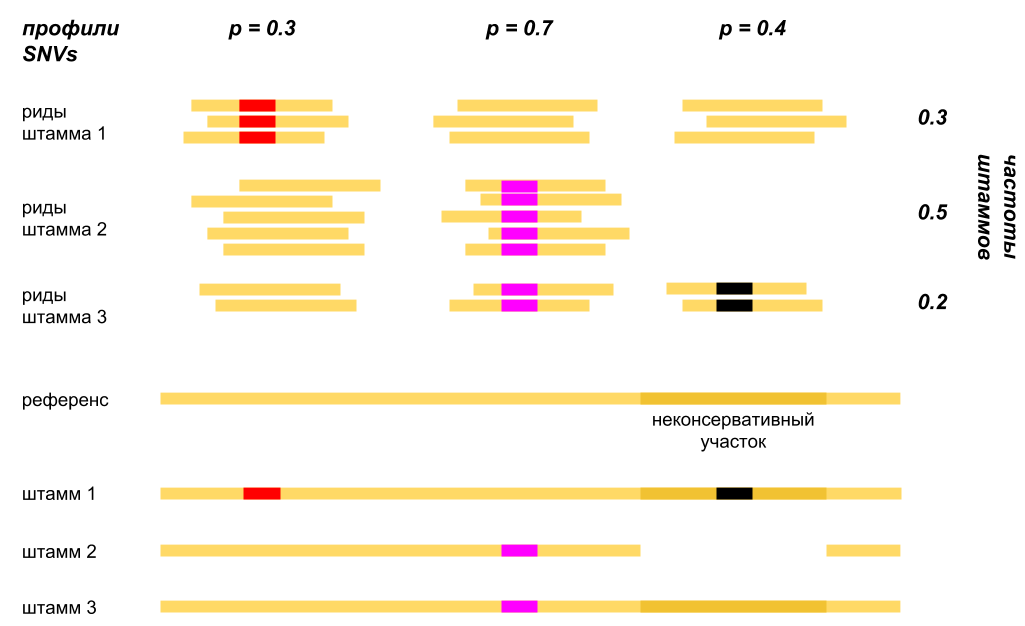
\includegraphics[width=0.9\textwidth]{pics/snv_profiles.png}
\caption{Подсчёт частот однонуклеотидныx мутаций (SNVs) для одного образца}
\label{snv_profile}
\end{figure}

DESMAN \cite{DESMAN} ищет в контигах однокопийные консервативные гены (те, которые должны присутствовать во всех штаммах рассматриваемого вида), и уже в них ищет SNVs. Затем он использует Байесовскую модель наподобие Lineage, но без учёта филогении, чтобы выяснить количество и частоты штаммов. После этого DESMAN выясняет, какому подмножеству штаммов принадлежит каждый из найденных неконсервативных генов (тех, которые могут отсутствовать в одном или нескольких штаммах). Таким образом, DESMAN --- это единственный из инструментов для анализа смесей штаммов в сериях \textit{de novo}, который выясняет не только профили встречаемости штаммов и однонуклеотидные мутации, но и информацию о геномном составе каждого их них.

Данная работа также посвящена выяснению состава каждого из смеси близкородственных штаммов в метагеномной серии, но с использованием помимо информации о профилях SNVs, еще и информации о структуре графа сборки. В графе сборке на основе графа де Брюйна \cite{de_Bruijn} вершины соответствуют фрагментам отсеквенированных геномов, а каждый геном представляет в графе связный путь. Таким образом граф даёт дополнительную информацию об устройстве геномов, которая потом теряется, если смотреть только на контиги. Кроме того свойства графа де Брюйна гарантируют нам, что фрагменты генома, соответствующие вершинам графа, не будут химерными (то есть ситуация, при которой разные части фрагмента принадлежат разным штаммам), в отличие от контигов.

На сегодняшний момент нам известен только один инструмент, использующий структуру графа сборки для анализа смесей близкородственных штаммов, --- это MaryGold \cite{MaryGold}, но он только ищет набор мест в графе, соответствующих вариациям между штаммами. Задачу, схожую по сути с поставленной, решают в транскриптомике при поиске изоформ гена \cite{flipflop2, other_flows, flipflop1}. Как в данной работе нам нужно определить, какому набору штаммов принадлежит геномный фрагмент, так при РНК-секвенировании нужно находить, из каких изоформ прочитался тот или иной экзон.

Таким образом целью данной работы является разработка пайплайна, который будет выявлять количество близкородственных штаммов в метагеномной серии, их процентное соотношение, а также для вершин графа сборки этих штаммов определять, какому подмножеству штаммов они принадлежат.


\section{Краткое описание подхода}

В данной работе мы будем анализировать графы сборки, полученные с помощью программы MetaSpades \cite{MetaSpades}. Вершины в таком графе соответствуют фрагментам геномов, а направленное ребро соединяет вершину $A$ с вершиной $B$ в том и только том случае, если последние $k$ нуклеотидов вершины $A$ равны первым $k$ нуклеотидам вершины $B$. Мы подобрали параметры этапа симлификации алгоритма (то есть, упрощения структуры графа) таким образом, чтобы из графа не выкидывались вершины, соответствующие недоминантным штаммам, стараясь сохранить таким образом свойство о том, что геному каждого штамма в графе соответствует связный путь. Но при этом мы соединяли в одну вершины, соответствующие однонуклеотидным мутациям или коротким вставкам/удалениям, чтобы граф не был слишком большим.

В основе первого этапа нашего алгоритма лежит метод DESMAN. Мы используем его для того, чтобы найти количество штаммов и их процентное соотношение, а также определить, каким штаммам принадлежат вершины графа сборки, соответствующие длинным фрагментам геномов. Эта первоначальная классификация является отправной точкой нашего дальнейшего алгоритма, в котором мы пытаемся классифицировать остальные вершины, основываясь уже на структуре графа.



\section{Классификация вершин с использованием DESMAN}


\subsection{Поиск SNVs}

Вначале нужно выравнять риды на референс, чтобы найти SNVs. В случае, когда уже известен геном хотя бы одного любого штамма интересующего вида, можно использовать его, так как референс нужен только для того, чтобы найти позиции, в которых присутствуют разные варианты нуклеотидов. В случае, если референс неизвестен, можно использовать длинные контиги, которые по результатам биннинга принадлежат интересующему виду. 

Для выравнивания ридов мы использовали программу BWA MEM ССЫЛКА. Для поиска SNVs --- инструмент VarScan ССЫЛКА; он позволяет не только находить позиции, в которых нуклеотиды отличаются от референса, но и проверять гипотезу о том, что это действительно мутация, а не ошибки секвенирования. 

Отдельно хотим отметить, что на этом этапе можно оценить, присутствует ли в принципе в образцах смесь близкородственных штаммов. ПРОДОЛЖИТЬ -- подробнее об этом в приложении ???

\subsection{Фильтрация SNVs}

Чтобы правильно вывести из частот SNVs частоты штаммов, нужно брать только те позиции в геноме, которые не попадают на плохо покрытые участки, не принадлежат повторам и при этом присутствуют во всех штаммах рассматриваемого вида (см. пример на Рис. \ref{snv_profile}). Чтобы выполнить последние два условия, DESMAN ищет в контигах однокопийные консервативные гены и рассматривает мутации только в них. Авторы предлагают самостоятельно составлять базу таких генов для видов с большим количеством известных геномов (в своей статье они нашли 900 ??? таких генов для E.Coli), а в случае, если доступных геномов мало, смотреть только на 36 генов, консервативных и однокопийных практически для всех эукариот. Но наши эксперименты (подробнее в ССЫЛКА) показали, что в случае, когда штаммы близкородственны, в этих 36 генов случается мало мутаций, и из-за этого результаты для профилей частот штаммов оказываются неудовлетворительными. Поэтому мы ищем мутации во всём геноме и после этого фильтруем их. 

Мы считаем медиану покрытия всех найденных позиций с SNVs в каждом образце, предполагая, что она отражает реальное покрытие всех штаммов рассматриваемого вида в совокупности. Таким образом нам нужны позиции с SNVs, суммарное покрытие которых близко к медиане в каждом из образцов. Поэтому мы считаем L2-расстояние между медианой и покрытием для каждой позиции и берём 3000 самых лучших (но это число можно менять в зависимости от условий, таких как степень родства штаммов и количество образцов).

\subsection{Количество штаммов и профили их частот}

Далее, имея вектора частот SNVs, мы можем вывести процентное соотношение с помощью одного из инструментов, упомянутых во введении. В данном случае мы используем DESMAN, как наиболее эффективный и строгий метод из всех доступных. Байесовская модель DESMAN предполагает знание количестве всех 4 нуклеотидов в рассматриваемых позициях --- эту информацию мы узнаём с помощью инструмента Bamreadcount. Другой инструмент, который можно применять для этого --- это MIDAS, но он подходит только в том случае, если в качестве референса берётся геном из его базы.

Для модели DESMAN количество штаммов в образцах является входным параметром алгоритма. Но авторы предлагают использовать график ??? для того, чтобы понять, начиная с какого количества штаммов ???? перестаёт значительно уменьшаться. Наши эксперименты показали, что этот метод работает как для симулированных, так и для реального датасетов.

\subsection{Классификация вершин графа сборки}

В оригинальной статье авторы DESMAN после выяснения профилей частот штаммов предлагают использовать это знания для классификации по штаммам неконсервативных генов на основе их покрытия, используя также Байесовский подход. Мы же в данной работе адаптировали данный алгоритм для геномных фрагментов, соответствующих длинным рёбрам в графе сборки, так как по сути для использования этого метода нам нужна только достоверная информация о покрытии фрагмента в каждом из образцов.

Алгоритм DESMAN не работает для повторов, но мы берём только длинные вершины.




\section{Валидация и типичные проблемы в результатах DESMAN}
\subsection{Описание датасетов}
\subsection{Описание способа валидации}
\subsection{Описание метрик}
\subsection{Результаты}


\section{Методы уточнения классификации с использованием структуры графа}
\subsection{Однозначное продолжение пути в графе}
\subsection{Пузыри в графе}
\subsection{Итоговый алгоритм}


\section{Результаты}
\subsection{Валидация результатов (прикладывание рёбер, описание метрик)}
\subsection{Простые датасеты из смесей изолятов}
\subsection{Датасет Strain Mock}
\subsection{Реальный датасет}







% У заключения нет номера главы
\section*{Заключение}
В данной работе 






\bibliographystyle{ugost2008ls}
\bibliography{diploma.bib}

\appendix

\section{приложение раз}
текст
\section{приложение два}
текст

\end{document}
